\documentclass[12pt, twoside]{article}
\usepackage{amsmath}
\usepackage{amssymb}
\usepackage{graphicx}
\usepackage{enumerate}
\usepackage{geometry}
\usepackage{pgfplots}
\pgfplotsset{compat=1.18}
\usepackage{tikz}
\geometry{margin=1in}

\begin{document}

\begin{center}
\Large{\textbf{IB Mathematics Standard Level}} \\
\large{\textbf{Paper 2}} \\
\normalsize{13 November 2018 -- Calculator Allowed} \\
\normalsize{90 marks total}
\end{center}

\vspace{0.5cm}

\section*{Section A}

\begin{enumerate}

% Question 1 [6 marks]
\item \textbf{[6 marks]} In a group of 35 students, some take art class ($A$) and some take music class ($M$). 5 of these students do not take either class. This information is shown in the following Venn diagram.

\begin{center}
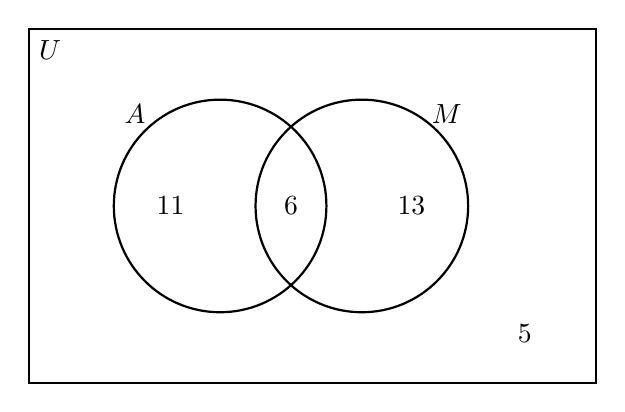
\begin{tikzpicture}[scale=0.9]
    % Universe rectangle
    \draw[thick] (-3.5,-2.5) rectangle (4.5,2.5);
    \node at (-3.2,2.2) {$U$};

    % Circle A
    \draw[thick] (-0.8,0) circle (1.5);
    \node at (-2,1.3) {$A$};

    % Circle M
    \draw[thick] (1.2,0) circle (1.5);
    \node at (2.4,1.3) {$M$};

    % Numbers in regions
    \node at (-1.5,0) {11};
    \node at (0.2,0) {6};
    \node at (1.9,0) {13};
    \node at (3.5,-1.8) {5};
\end{tikzpicture}
\end{center}

\begin{enumerate}[(a)]
    \item Write down the number of students in the group who take art class.
    \item One student from the group is chosen at random. Find the probability that
    \begin{enumerate}[(i)]
        \item the student does not take art class;
        \item the student takes either art class or music class, but not both.
    \end{enumerate}
\end{enumerate}

\vspace{1cm}

% Question 2 [6 marks]
\item \textbf{[6 marks]} The following table shows the hand lengths and the heights of five athletes on a sports team.

\begin{center}
\begin{tabular}{|c|c|c|c|c|c|}
\hline
\textbf{Hand length ($x$ cm)} & 21.0 & 21.9 & 21.0 & 20.3 & 20.8 \\
\hline
\textbf{Height ($y$ cm)} & 178.3 & 185.0 & 177.1 & 169.0 & 174.6 \\
\hline
\end{tabular}
\end{center}

The relationship between $x$ and $y$ can be modelled by the regression line with equation $y = ax + b$.

\begin{enumerate}[(a)]
    \item \begin{enumerate}[(i)]
        \item Find the value of $a$ and of $b$.
        \item Write down the correlation coefficient.
    \end{enumerate}
    \item Another athlete on this sports team has a hand length of 21.5\,cm. Use the regression equation to estimate the height of this athlete.
\end{enumerate}

\vspace{1cm}

% Question 3 [7 marks]
\item \textbf{[7 marks]} Let $f(x) = \dfrac{6x-1}{2x+3}$, for $x \neq -\dfrac{3}{2}$.

\begin{enumerate}[(a)]
    \item For the graph of $f$,
    \begin{enumerate}[(i)]
        \item find the $y$-intercept;
        \item find the equation of the vertical asymptote;
        \item find the equation of the horizontal asymptote.
    \end{enumerate}
    \item Hence or otherwise, write down $\displaystyle\lim_{x \to \infty} \left(\frac{6x-1}{2x+3}\right)$.
\end{enumerate}

\vspace{1cm}

% Question 4 [7 marks]
\item \textbf{[7 marks]} A particle moves along a straight line so that its velocity, $v$\,ms$^{-1}$, after $t$ seconds is given by $v(t) = 1.4^t - 2.7$, for $0 \leq t \leq 5$.

\begin{enumerate}[(a)]
    \item Find when the particle is at rest.
    \item Find the acceleration of the particle when $t = 2$.
    \item Find the total distance travelled by the particle.
\end{enumerate}

\vspace{1cm}

% Question 5 [6 marks]
\item \textbf{[6 marks]} The sum of an infinite geometric sequence is 33.25. The second term of the sequence is 7.98. Find the possible values of $r$.

\vspace{1cm}

% Question 6 [7 marks]
\item \textbf{[7 marks]} Consider the expansion of $\left(2x^4 + \dfrac{x^2}{k}\right)^{12}$, $k \neq 0$. The coefficient of the term in $x^{40}$ is five times the coefficient of the term in $x^{38}$. Find $k$.

\vspace{1cm}

% Question 7 [6 marks]
\item \textbf{[6 marks]} A communication tower, T, produces a signal that can reach cellular phones within a radius of 32\,km. A straight road passes through the area covered by the tower's signal.

The following diagram shows a line representing the road and a circle representing the area covered by the tower's signal. Point R is on the circumference of the circle and points S and R are on the road. Point S is 38\,km from the tower and $\mathrm{R\hat{S}T} = 43°$.

\begin{center}
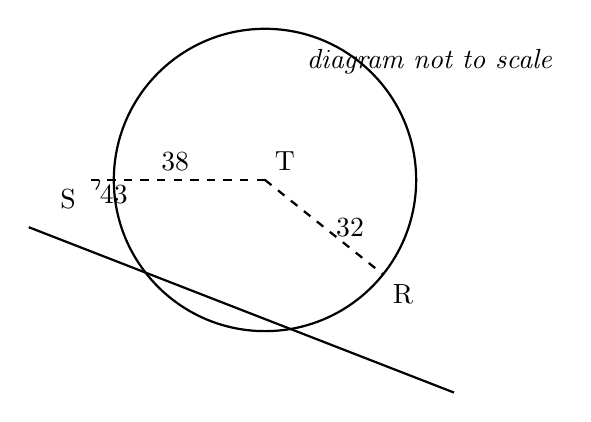
\begin{tikzpicture}[scale=0.06]
    % Circle for tower coverage
    \draw[thick] (0,0) circle (32);

    % Tower point T
    \fill (0,0) circle (8pt) node[above right] {T};

    % Point S outside circle
    \coordinate (S) at (-38,0);

    % Calculate intersection points with circle
    % Road goes from S at angle 43 degrees
    % Line: y = tan(43°)(x + 38)
    % Circle: x^2 + y^2 = 32^2

    % Point R on circle (approximate)
    \coordinate (R) at (25,-20);

    % Draw road line through S
    \draw[thick] (-50,-10) -- (40,-45);

    % Draw radius to R
    \draw[thick, dashed] (0,0) -- (25,-20);

    % Draw ST
    \draw[thick, dashed] (0,0) -- (-38,0);

    % Labels
    \node[below left] at (-38,0) {S};
    \node[below right] at (25,-20) {R};

    % Angle arc at S
    \draw (-35,0) arc (0:-43:3);
    \node at (-32,-3) {$43°$};

    % Distance labels
    \node[above] at (-19,0) {38};
    \node[right] at (13,-10) {32};

    % Note
    \node at (35,25) {\textit{diagram not to scale}};
\end{tikzpicture}
\end{center}

\begin{enumerate}[(a)]
    \item Let SR $= x$. Use the cosine rule to show that $x^2 - (76\cos 43)x + 420 = 0$.
    \item Hence or otherwise, find the total distance along the road where the signal from the tower can reach cellular phones.
\end{enumerate}

\newpage

\section*{Section B}

\setcounter{enumi}{7}

% Question 8 [16 marks]
\item \textbf{[16 marks]} Consider the points A$(-3, 4, 2)$ and B$(8, -1, 5)$.

\begin{enumerate}[(a)]
    \item \begin{enumerate}[(i)]
        \item Find $\overrightarrow{\mathrm{AB}}$.
        \item Find $\left|\overrightarrow{\mathrm{AB}}\right|$.
    \end{enumerate}
\end{enumerate}

A line $L$ has vector equation $\mathbf{r} = \begin{pmatrix} 2 \\ 0 \\ -5 \end{pmatrix} + t\begin{pmatrix} 1 \\ -2 \\ 2 \end{pmatrix}$. The point C$(5, y, 1)$ lies on line $L$.

\begin{enumerate}[(a)]
    \setcounter{enumii}{1}
    \item \begin{enumerate}[(i)]
        \item Find the value of $y$.
        \item Show that $\overrightarrow{\mathrm{AC}} = \begin{pmatrix} 8 \\ -10 \\ -1 \end{pmatrix}$.
    \end{enumerate}
    \item Find the angle between $\overrightarrow{\mathrm{AB}}$ and $\overrightarrow{\mathrm{AC}}$.
    \item Find the area of triangle ABC.
\end{enumerate}

\vspace{1cm}

% Question 9 [15 marks]
\item \textbf{[15 marks]} A nationwide study on reaction time is conducted on participants in two age groups. The participants in Group X are less than 40 years old. Their reaction times are normally distributed with mean 0.489 seconds and standard deviation 0.07 seconds.

\begin{enumerate}[(a)]
    \item A person is selected at random from Group X. Find the probability that their reaction time is greater than 0.65 seconds.
\end{enumerate}

The participants in Group Y are 40 years or older. Their reaction times are normally distributed with mean 0.592 seconds and standard deviation $\sigma$ seconds.

\begin{enumerate}[(a)]
    \setcounter{enumii}{1}
    \item The probability that the reaction time of a person in Group Y is greater than 0.65 seconds is 0.396. Find the value of $\sigma$.
\end{enumerate}

In the study, 38\% of the participants are in Group X.

\begin{enumerate}[(a)]
    \setcounter{enumii}{2}
    \item A randomly selected participant has a reaction time greater than 0.65 seconds. Find the probability that the participant is in Group X.
    \item Ten of the participants with reaction times greater than 0.65 are selected at random. Find the probability that at least two of them are in Group X.
\end{enumerate}

\vspace{1cm}

% Question 10 [14 marks]
\item \textbf{[14 marks]} All lengths in this question are in metres.

Consider the function $f(x) = \sqrt{\dfrac{4-x^2}{8}}$, for $-2 \leq x \leq 2$. In the following diagram, the shaded region is enclosed by the graph of $f$ and the $x$-axis.

\begin{center}
\begin{tikzpicture}
\begin{axis}[
    width=10cm,
    height=6cm,
    axis lines=middle,
    xlabel={$x$},
    ylabel={$y$},
    xmin=-3, xmax=3,
    ymin=-0.3, ymax=1,
    xtick={-2,2},
    ytick={},
    samples=100,
    smooth,
]
% f(x) = sqrt((4-x^2)/8)
\addplot[domain=-2:2, blue, thick, name path=curve] {sqrt((4-x^2)/8)};
\addplot[domain=-2:2, draw=none, name path=axis] {0};
% s\addplot[gray!30] fill between[of=curve and axis];
\end{axis}
\node at (5.5,3.5) {\textit{diagram not to scale}};
\end{tikzpicture}
\end{center}

A container can be modelled by rotating this region by $360$ about the $x$-axis.

\begin{enumerate}[(a)]
    \item Find the volume of the container.
\end{enumerate}

Water can flow in and out of the container.

The volume of water in the container is given by the function $g(t)$, for $0 \leq t \leq 4$, where $t$ is measured in hours and $g(t)$ is measured in m$^3$. The rate of change of the volume of water in the container is given by $g'(t) = 0.9 - 2.5\cos(0.4t^2)$.

\begin{enumerate}[(a)]
    \setcounter{enumii}{1}
    \item The volume of water in the container is increasing only when $p < t < q$.
    \begin{enumerate}[(i)]
        \item Find the value of $p$ and of $q$.
        \item During the interval $p < t < q$, the volume of water in the container increases by $k$\,m$^3$. Find the value of $k$.
    \end{enumerate}
\end{enumerate}

When $t = 0$, the volume of water in the container is 2.3\,m$^3$. It is known that the container is never completely full of water during the 4 hour period.

\begin{enumerate}[(a)]
    \setcounter{enumii}{2}
    \item Find the minimum volume of empty space in the container during the 4 hour period.
\end{enumerate}

\end{enumerate}

\end{document}
